\documentclass{article}

% Language setting
% Replace `english' with e.g. `spanish' to change the document language
\usepackage[UTF8]{ctex}

% Set page size and margins
% Replace `letterpaper' with `a4paper' for UK/EU standard size
\usepackage[letterpaper,top=2cm,bottom=2cm,left=3cm,right=3cm,marginparwidth=1.75cm]{geometry}

% Useful packages
\usepackage{amsmath}
\usepackage{graphicx}
\usepackage[colorlinks=true, allcolors=blue]{hyperref}

\title{MA206 Homework4}
\author{12110120 赵钊}

\begin{document}
\maketitle


\section{第1题}

\begin{table}[!h]
\begin{center}
\begin{tabular}{ c c c }
    \hline
    Planet & Period(T) & Mean distance from the sun(r)\\
    \hline
    Mercury & 88 & 57.9\\
    Venus & 225 & 108.2\\ 
    Earth & 365 & 149.6\\ 
    Mars & 687 & 227.9\\ 
    Jupiter & 4329 & 778.1\\
    Saturn & 10753 & 1428.2\\
    Uranus & 30660 & 2837.9\\
    Neptune & 60150 & 4488.9\\
    \hline
\end{tabular}
\caption{\label{demo-table}行星数据}
\end{center}
\end{table}

对上表数据运用Matlab进行绘图,绘制的散点图如下

\begin{figure}[!h]
    \centering
    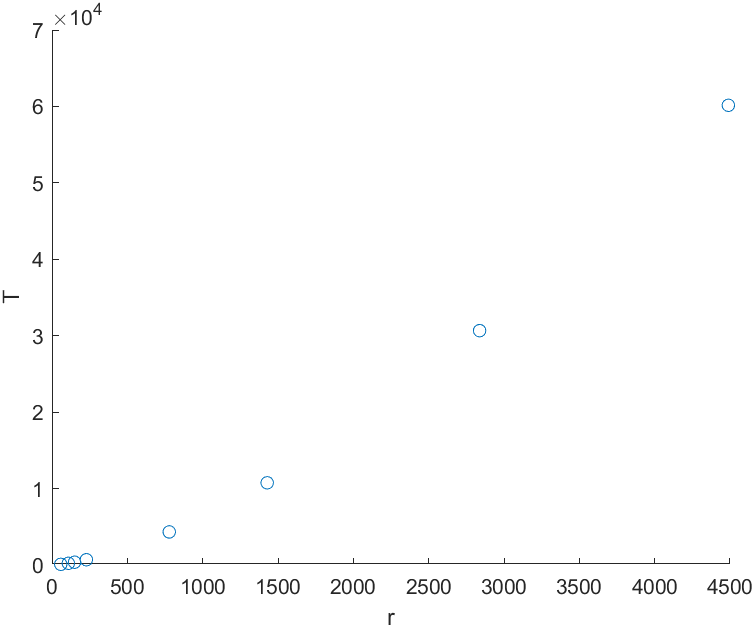
\includegraphics[width=0.6\textwidth]{picture/hw4_1.png}
    \caption{r-T图}
\end{figure}

\newpage

对数据进行取对数处理

\begin{table}[!h]
\begin{center}
\begin{tabular}{|c|c|c|c|c|c|c|c|c|}
    \hline
    $lnT$ & 4.48 & 5.42 & 5.90 & 6.53 & 8.37 & 9.28 & 10.3 & 11.0   \\
    \hline
    $lnr$ & 4.06 & 4.68 & 5.01 & 5.43 & 6.66 & 7.26 & 7.95 & 8.41   \\
    \hline
\end{tabular}
\caption{\label{demo-table}取对数}
\end{center}
\end{table}

\begin{figure}[!h]
    \centering
    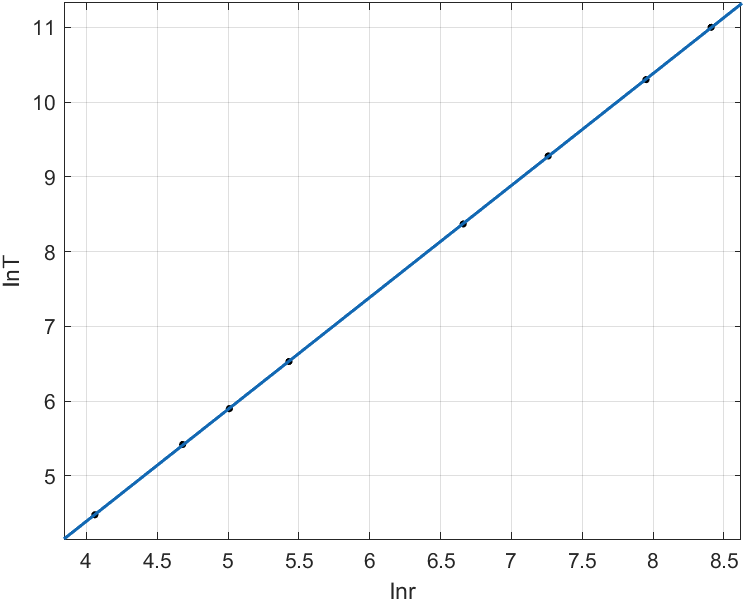
\includegraphics[width=0.6\textwidth]{picture/hw4_2.png}
    \caption{拟合}
\end{figure}

对数据进行线性最小二乘拟合,得到的线性方程为
\[lnT = 1.497lnr - 1.597  \quad (R^2 = 1)\]

即
\[T = e^{-1.597}r^{1.497} \approx 0.203r^{1.5}\]

对比开普勒第三定律
\[\frac{T^2}{r^3} = const\]

发现基本吻合

\newpage

\section{第2题}

对数据进行取对数处理

\begin{table}[!h]
\begin{center}
\begin{tabular}{|c|c|c|c|}
    \hline
    $V$ & $lnV$ & $P$ & $lnP$ \\
    \hline
    2.27 & 0.82 & 2500 & 7.82\\
    \hline
    2.76 & 1.02 & 365 & 5.90\\
    \hline
    3.27 & 1.18 & 23700 & 10.07\\
    \hline
    3.31 & 1.20 & 5491 & 8.61\\
    \hline
    3.70 & 1.31 & 14000 & 9.55\\
    \hline
    3.85 & 1.35 & 78200 & 11.27\\
    \hline
    4.31 & 1.46 & 70700 & 11.17\\
    \hline
    4.39 & 1.48 & 138000 & 11.84\\
    \hline
    4.42 & 1.49 & 304500 & 12.63\\
    \hline
    4.81 & 1.57 & 341948 & 12.74\\
    \hline
    4.90 & 1.59 & 49375 & 10.81\\
    \hline
    5.05 & 1.62 & 260200 & 12.47\\
    \hline
    5.21 & 1.65 & 867023 & 13.67\\
    \hline
    5.62 & 1.73 & 1340000 & 14.11\\
    \hline
    5.88 & 1.77 & 1092759 & 13.90\\
    \hline
\end{tabular}
\caption{\label{demo-table}数据处理}
\end{center}
\end{table}

\begin{figure}[!h]
    \centering
    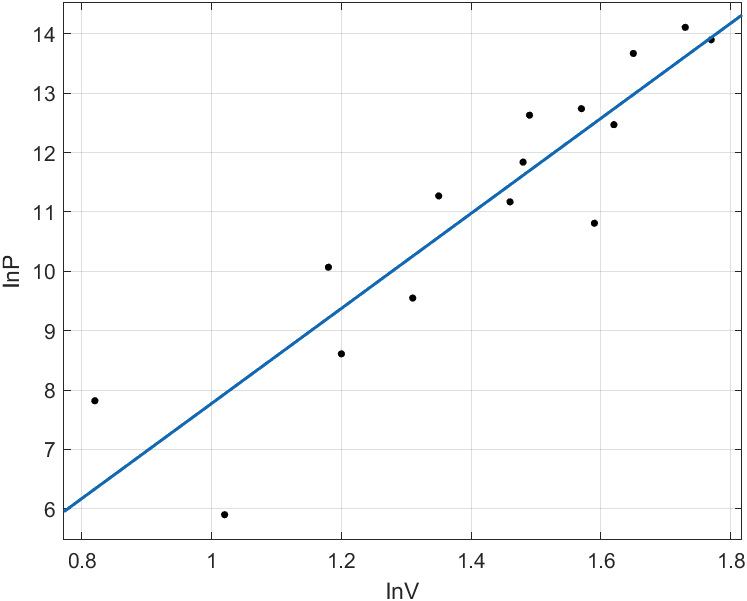
\includegraphics[width=0.5\textwidth]{picture/hw4_3.png}
    \caption{拟合}
\end{figure}

对$lnV$和$lnP$进行线性拟合得到
\[lnP = 8.005lnV - 0.2309 \quad  (R_1^2 = 0.8287)\]

即
\[P = e^{-0.2309}V^{8.005} \approx 0.794V^{8.005}\]

\begin{figure}[!h]
    \centering
    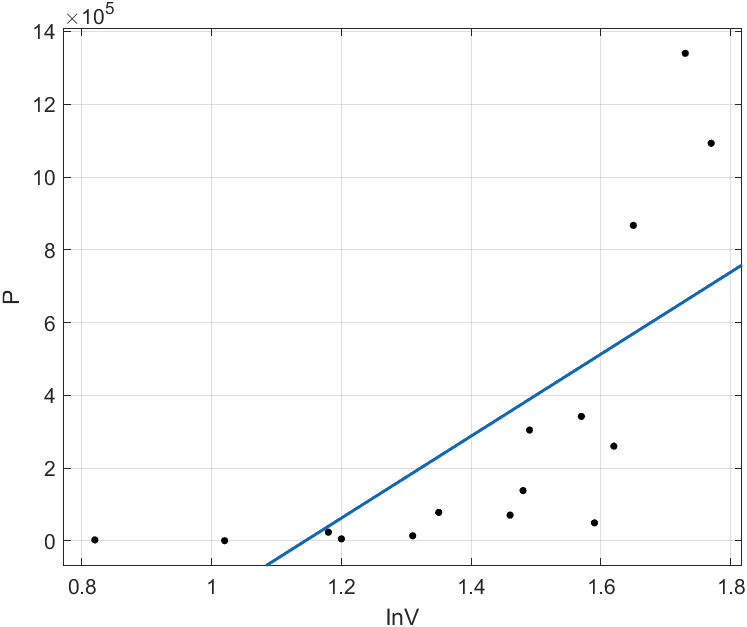
\includegraphics[width=0.5\textwidth]{picture/hw4_4.png}
    \caption{拟合}
\end{figure}

对$lnV$和$P$进行线性拟合得到
\[P = 1.13 \times 10^6 lnV - 1.29 \times 10^6 \quad (R_2^2 = 0.4867)\]

比较发现,$R_1^2>R^2_2$,因此选择$P=aV^b$的模型进行拟合更优.


\section{第3题}
以$a$和$b$作为变量,求解原方程组
\[
\begin{cases}
(\sum x_i^2)a + (\sum x_i)b = \sum x_iy_i & (1)
\\
(\sum x_i)a + mb = \sum y_i & (2)
\end{cases} 
\]

$(1) \times m$、$(2) \times \sum x_i$ 可得
\[
\begin{cases}
m(\sum x_i^2)a + m(\sum x_i)b = m\sum x_iy_i & (3)
\\
(\sum x_i)^2a + m(\sum x_i)b = \sum x_i \sum y_i & (4)
\end{cases} 
\]

$(3) - (4)$有
\[[m\sum x_i^2 - (\sum x_i)^2]a = m\sum x_iy_i - \sum x_i \sum y_i\]

即
\[a = \frac{m\sum x_iy_i - \sum x_i \sum y_i}{m\sum x_i^2 - (\sum x_i)^2}\]

代入$(2)$可得
\[
mb = \sum y_i - \sum x_i \frac{m\sum x_iy_i - \sum x_i \sum y_i}{m\sum x_i^2 - (\sum x_i)^2}
\]

化简得
\[b = \frac{\sum x_i^2 \sum y_i - \sum x_iy_i \sum x_i}{m\sum x_i^2 - (\sum x_i)^2}\]


\newpage

\section{第4题}

\begin{table}[!h]
\begin{center}
\begin{tabular}{c|c c c c c c c c c c c c c c}
    x & 17 & 19 & 20 & 22 & 23 & 25 & 28 & 31 & 32 & 33 & 36 & 37 & 39 & 42   \\
    \hline
    y & 19 & 25 & 32 & 51 & 57 & 71 & 113 & 140 & 153 & 187 & 192 & 205 & 250 & 260  \\
\end{tabular}
\caption{\label{demo-table}第4题数据}
\end{center}
\end{table}

\subsection{a}
\begin{figure}[!h]
    \centering
    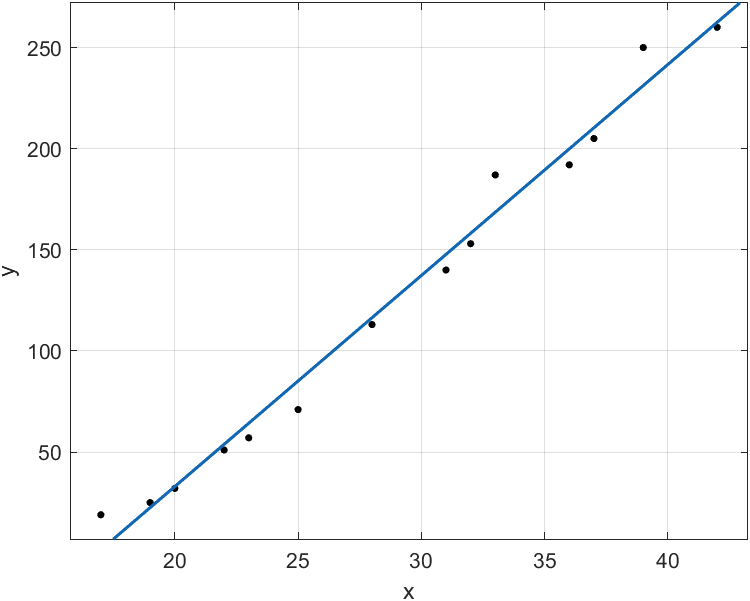
\includegraphics[width=0.5\textwidth]{picture/hw4_5.png}
    \caption{拟合}
\end{figure}

结果为$y = 10.43x - 175.7$

\subsection{b}
\begin{figure}[!h]
    \centering
    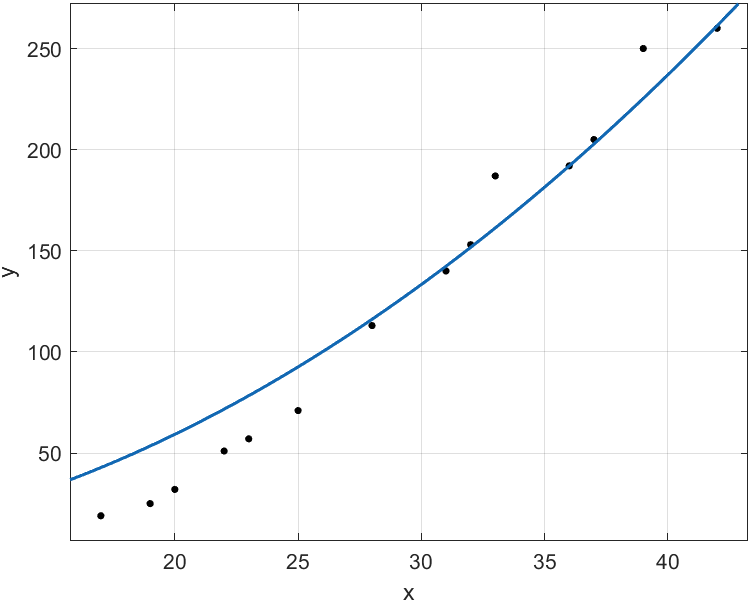
\includegraphics[width=0.5\textwidth]{picture/hw4_6.png}
    \caption{拟合}
\end{figure}

结果为$y = 0.1481x^2$

\subsection{c}
\begin{figure}[!h]
    \centering
    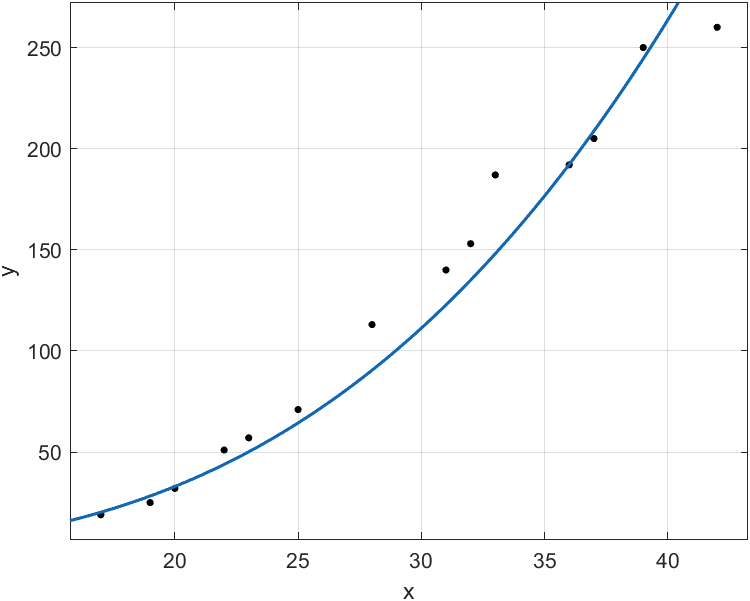
\includegraphics[width=0.5\textwidth]{picture/hw4_7.png}
    \caption{拟合}
\end{figure}

结果为$y = 0.00412x^3$

\subsection{d}
\begin{figure}[!h]
    \centering
    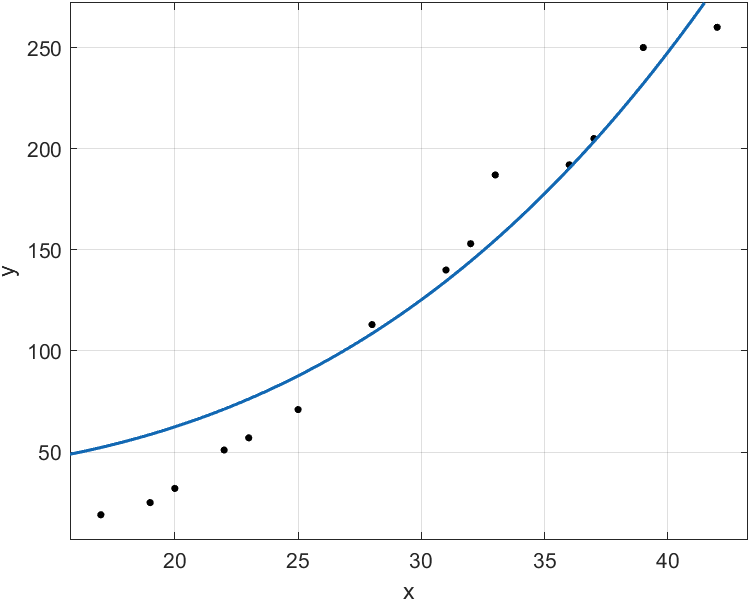
\includegraphics[width=0.5\textwidth]{picture/hw4_8.png}
    \caption{拟合}
\end{figure}

结果为$y = 0.003307x^3 - 2.252x^2 + 30.93$

\end{document}
